\documentclass[1p]{elsarticle_modified}
%\bibliographystyle{elsarticle-num}

%\usepackage[colorlinks]{hyperref}
%\usepackage{abbrmath_seonhwa} %\Abb, \Ascr, \Acal ,\Abf, \Afrak
\usepackage{amsfonts}
\usepackage{amssymb}
\usepackage{amsmath}
\usepackage{amsthm}
\usepackage{scalefnt}
\usepackage{amsbsy}
\usepackage{kotex}
\usepackage{caption}
\usepackage{subfig}
\usepackage{color}
\usepackage{graphicx}
\usepackage{xcolor} %% white, black, red, green, blue, cyan, magenta, yellow
\usepackage{float}
\usepackage{setspace}
\usepackage{hyperref}

\usepackage{tikz}
\usetikzlibrary{arrows}

\usepackage{multirow}
\usepackage{array} % fixed length table
\usepackage{hhline}

%%%%%%%%%%%%%%%%%%%%%
\makeatletter
\renewcommand*\env@matrix[1][\arraystretch]{%
	\edef\arraystretch{#1}%
	\hskip -\arraycolsep
	\let\@ifnextchar\new@ifnextchar
	\array{*\c@MaxMatrixCols c}}
\makeatother %https://tex.stackexchange.com/questions/14071/how-can-i-increase-the-line-spacing-in-a-matrix
%%%%%%%%%%%%%%%

\usepackage[normalem]{ulem}

\newcommand{\msout}[1]{\ifmmode\text{\sout{\ensuremath{#1}}}\else\sout{#1}\fi}
%SOURCE: \msout is \stkout macro in https://tex.stackexchange.com/questions/20609/strikeout-in-math-mode

\newcommand{\cancel}[1]{
	\ifmmode
	{\color{red}\msout{#1}}
	\else
	{\color{red}\sout{#1}}
	\fi
}

\newcommand{\add}[1]{
	{\color{blue}\uwave{#1}}
}

\newcommand{\replace}[2]{
	\ifmmode
	{\color{red}\msout{#1}}{\color{blue}\uwave{#2}}
	\else
	{\color{red}\sout{#1}}{\color{blue}\uwave{#2}}
	\fi
}

\newcommand{\Sol}{\mathcal{S}} %segment
\newcommand{\D}{D} %diagram
\newcommand{\A}{\mathcal{A}} %arc


%%%%%%%%%%%%%%%%%%%%%%%%%%%%%5 test

\def\sl{\operatorname{\textup{SL}}(2,\Cbb)}
\def\psl{\operatorname{\textup{PSL}}(2,\Cbb)}
\def\quan{\mkern 1mu \triangleright \mkern 1mu}

\theoremstyle{definition}
\newtheorem{thm}{Theorem}[section]
\newtheorem{prop}[thm]{Proposition}
\newtheorem{lem}[thm]{Lemma}
\newtheorem{ques}[thm]{Question}
\newtheorem{cor}[thm]{Corollary}
\newtheorem{defn}[thm]{Definition}
\newtheorem{exam}[thm]{Example}
\newtheorem{rmk}[thm]{Remark}
\newtheorem{alg}[thm]{Algorithm}

\newcommand{\I}{\sqrt{-1}}
\begin{document}

%\begin{frontmatter}
%
%\title{Boundary parabolic representations of knots up to 8 crossings}
%
%%% Group authors per affiliation:
%\author{Yunhi Cho} 
%\address{Department of Mathematics, University of Seoul, Seoul, Korea}
%\ead{yhcho@uos.ac.kr}
%
%
%\author{Seonhwa Kim} %\fnref{s_kim}}
%\address{Center for Geometry and Physics, Institute for Basic Science, Pohang, 37673, Korea}
%\ead{ryeona17@ibs.re.kr}
%
%\author{Hyuk Kim}
%\address{Department of Mathematical Sciences, Seoul National University, Seoul 08826, Korea}
%\ead{hyukkim@snu.ac.kr}
%
%\author{Seokbeom Yoon}
%\address{Department of Mathematical Sciences, Seoul National University, Seoul, 08826,  Korea}
%\ead{sbyoon15@snu.ac.kr}
%
%\begin{abstract}
%We find all boundary parabolic representation of knots up to 8 crossings.
%
%\end{abstract}
%\begin{keyword}
%    \MSC[2010] 57M25 
%\end{keyword}
%
%\end{frontmatter}

%\linenumbers
%\tableofcontents
%
\newcommand\colored[1]{\textcolor{white}{\rule[-0.35ex]{0.8em}{1.4ex}}\kern-0.8em\color{red} #1}%
%\newcommand\colored[1]{\textcolor{white}{ #1}\kern-2.17ex	\textcolor{white}{ #1}\kern-1.81ex	\textcolor{white}{ #1}\kern-2.15ex\color{red}#1	}

{\Large $\underline{12a_{0002}~(K12a_{0002})}$}

\setlength{\tabcolsep}{10pt}
\renewcommand{\arraystretch}{1.6}
\vspace{1cm}\begin{tabular}{m{100pt}>{\centering\arraybackslash}m{274pt}}
\multirow{5}{120pt}{
	\centering
	\includegraphics[width=112pt]{../../../GIT/diagram.site/Diagrams/png/803_12a_0002.png}\\
\ \ \ A knot diagram\footnotemark}&
\allowdisplaybreaks
\textbf{Linearized knot diagam} \\
\cline{2-2}
 &
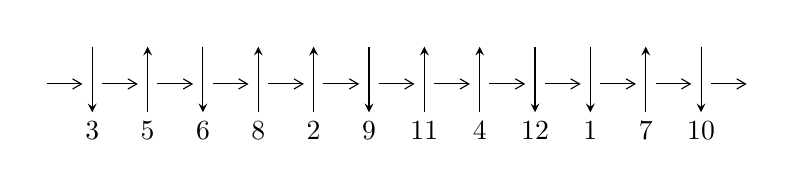
\begin{tikzpicture}[x=20pt, y=17pt]
	% nodes
	\node (C0) at (0, 0) {};
	\node (C1) at (1, 0) {};
	\node (C1U) at (1, +1) {};
	\node (C1D) at (1, -1) {3};

	\node (C2) at (2, 0) {};
	\node (C2U) at (2, +1) {};
	\node (C2D) at (2, -1) {5};

	\node (C3) at (3, 0) {};
	\node (C3U) at (3, +1) {};
	\node (C3D) at (3, -1) {6};

	\node (C4) at (4, 0) {};
	\node (C4U) at (4, +1) {};
	\node (C4D) at (4, -1) {8};

	\node (C5) at (5, 0) {};
	\node (C5U) at (5, +1) {};
	\node (C5D) at (5, -1) {2};

	\node (C6) at (6, 0) {};
	\node (C6U) at (6, +1) {};
	\node (C6D) at (6, -1) {9};

	\node (C7) at (7, 0) {};
	\node (C7U) at (7, +1) {};
	\node (C7D) at (7, -1) {11};

	\node (C8) at (8, 0) {};
	\node (C8U) at (8, +1) {};
	\node (C8D) at (8, -1) {4};

	\node (C9) at (9, 0) {};
	\node (C9U) at (9, +1) {};
	\node (C9D) at (9, -1) {12};

	\node (C10) at (10, 0) {};
	\node (C10U) at (10, +1) {};
	\node (C10D) at (10, -1) {1};

	\node (C11) at (11, 0) {};
	\node (C11U) at (11, +1) {};
	\node (C11D) at (11, -1) {7};

	\node (C12) at (12, 0) {};
	\node (C12U) at (12, +1) {};
	\node (C12D) at (12, -1) {10};
	\node (C13) at (13, 0) {};

	% arrows
	\draw[->,>={angle 60}]
	(C0) edge (C1) (C1) edge (C2) (C2) edge (C3) (C3) edge (C4) (C4) edge (C5) (C5) edge (C6) (C6) edge (C7) (C7) edge (C8) (C8) edge (C9) (C9) edge (C10) (C10) edge (C11) (C11) edge (C12) (C12) edge (C13) ;	\draw[->,>=stealth]
	(C1U) edge (C1D) (C2D) edge (C2U) (C3U) edge (C3D) (C4D) edge (C4U) (C5D) edge (C5U) (C6U) edge (C6D) (C7D) edge (C7U) (C8D) edge (C8U) (C9U) edge (C9D) (C10U) edge (C10D) (C11D) edge (C11U) (C12U) edge (C12D) ;
	\end{tikzpicture} \\
\hhline{~~} \\& 
\textbf{Solving Sequence} \\ \cline{2-2} 
 &
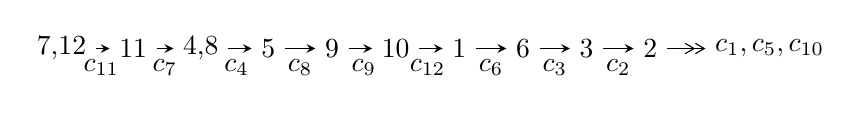
\begin{tikzpicture}[x=23pt, y=7pt]
	% node
	\node (A0) at (-1/8, 0) {7,12};
	\node (A1) at (1, 0) {11};
	\node (A2) at (33/16, 0) {4,8};
	\node (A3) at (25/8, 0) {5};
	\node (A4) at (33/8, 0) {9};
	\node (A5) at (41/8, 0) {10};
	\node (A6) at (49/8, 0) {1};
	\node (A7) at (57/8, 0) {6};
	\node (A8) at (65/8, 0) {3};
	\node (A9) at (73/8, 0) {2};
	\node (C1) at (1/2, -1) {$c_{11}$};
	\node (C2) at (3/2, -1) {$c_{7}$};
	\node (C3) at (21/8, -1) {$c_{4}$};
	\node (C4) at (29/8, -1) {$c_{8}$};
	\node (C5) at (37/8, -1) {$c_{9}$};
	\node (C6) at (45/8, -1) {$c_{12}$};
	\node (C7) at (53/8, -1) {$c_{6}$};
	\node (C8) at (61/8, -1) {$c_{3}$};
	\node (C9) at (69/8, -1) {$c_{2}$};
	\node (A10) at (11, 0) {$c_{1},c_{5},c_{10}$};

	% edge
	\draw[->,>=stealth]	
	(A0) edge (A1) (A1) edge (A2) (A2) edge (A3) (A3) edge (A4) (A4) edge (A5) (A5) edge (A6) (A6) edge (A7) (A7) edge (A8) (A8) edge (A9) ;
	\draw[->>,>={angle 60}]	
	(A9) edge (A10);
\end{tikzpicture} \\ 

\end{tabular} \\

\footnotetext{
The image of knot diagram is generated by the software ``\textbf{Draw programme}" developed by Andrew Bartholomew(\url{http://www.layer8.co.uk/maths/draw/index.htm\#Running-draw}), where we modified some parts for our purpose(\url{https://github.com/CATsTAILs/LinksPainter}).
}\phantom \\ \newline 
\centering \textbf{Ideals for irreducible components\footnotemark of $X_{\text{par}}$} 
 
\begin{align*}
I^u_{1}&=\langle 
2.87313\times10^{334} u^{104}-9.21887\times10^{334} u^{103}+\cdots+1.15405\times10^{337} b+3.50101\times10^{336},\\
\phantom{I^u_{1}}&\phantom{= \langle  }-2.56029\times10^{334} u^{104}+5.49406\times10^{334} u^{103}+\cdots+6.59460\times10^{336} a-2.98633\times10^{337},\\
\phantom{I^u_{1}}&\phantom{= \langle  }u^{105}-3 u^{104}+\cdots+2048 u+1024\rangle \\
I^u_{2}&=\langle 
- u^2 a+b- a,\;u^4 a+u^3 a+u^4+2 u^2 a+a^2+a u+u^2+a- u,\;u^5+u^4+2 u^3+u^2+u+1\rangle \\
\\
I^v_{1}&=\langle 
a,\;v^3+2 v^2+b+2 v,\;v^4+2 v^3+3 v^2+v+1\rangle \\
I^v_{2}&=\langle 
a,\;- v^3- v^2+b+1,\;v^6+3 v^5+4 v^4+2 v^3+1\rangle \\
\end{align*}
\raggedright * 4 irreducible components of $\dim_{\mathbb{C}}=0$, with total 125 representations.\\
\footnotetext{All coefficients of polynomials are rational numbers. But the coefficients are sometimes approximated in decimal forms when there is not enough margin.}
\newpage
\renewcommand{\arraystretch}{1}
\centering \section*{I. $I^u_{1}= \langle 2.87\times10^{334} u^{104}-9.22\times10^{334} u^{103}+\cdots+1.15\times10^{337} b+3.50\times10^{336},\;-2.56\times10^{334} u^{104}+5.49\times10^{334} u^{103}+\cdots+6.59\times10^{336} a-2.99\times10^{337},\;u^{105}-3 u^{104}+\cdots+2048 u+1024 \rangle$}
\flushleft \textbf{(i) Arc colorings}\\
\begin{tabular}{m{7pt} m{180pt} m{7pt} m{180pt} }
\flushright $a_{7}=$&$\begin{pmatrix}0\\u\end{pmatrix}$ \\
\flushright $a_{12}=$&$\begin{pmatrix}1\\0\end{pmatrix}$ \\
\flushright $a_{11}=$&$\begin{pmatrix}1\\u^2\end{pmatrix}$ \\
\flushright $a_{4}=$&$\begin{pmatrix}0.00388240 u^{104}-0.00833116 u^{103}+\cdots+11.4924 u+4.52845\\-0.00248959 u^{104}+0.00798824 u^{103}+\cdots-4.48147 u-0.303366\end{pmatrix}$ \\
\flushright $a_{8}=$&$\begin{pmatrix}u\\u^3+u\end{pmatrix}$ \\
\flushright $a_{5}=$&$\begin{pmatrix}0.00498777 u^{104}-0.0112515 u^{103}+\cdots+14.7026 u+5.39070\\-0.00215259 u^{104}+0.00751970 u^{103}+\cdots-3.21368 u+0.153629\end{pmatrix}$ \\
\flushright $a_{9}=$&$\begin{pmatrix}-0.000519769 u^{104}+0.00481996 u^{103}+\cdots+4.67049 u+3.48978\\-0.00119259 u^{104}+0.00216389 u^{103}+\cdots-4.22800 u-2.41288\end{pmatrix}$ \\
\flushright $a_{10}=$&$\begin{pmatrix}0.000672817 u^{104}+0.00265608 u^{103}+\cdots+8.89849 u+5.90266\\-0.00119259 u^{104}+0.00216389 u^{103}+\cdots-4.22800 u-2.41288\end{pmatrix}$ \\
\flushright $a_{1}=$&$\begin{pmatrix}0.000672817 u^{104}+0.00265608 u^{103}+\cdots+8.89849 u+5.90266\\-0.00129632 u^{104}+0.00157290 u^{103}+\cdots-6.03440 u-2.37383\end{pmatrix}$ \\
\flushright $a_{6}=$&$\begin{pmatrix}-0.00489883 u^{104}+0.0141883 u^{103}+\cdots-8.53327 u-2.46195\\0.00235848 u^{104}-0.00763297 u^{103}+\cdots+4.80576 u+0.638462\end{pmatrix}$ \\
\flushright $a_{3}=$&$\begin{pmatrix}-0.00606696 u^{104}+0.0253348 u^{103}+\cdots+2.81502 u+4.85586\\0.00220680 u^{104}-0.0101609 u^{103}+\cdots-3.08436 u-1.82736\end{pmatrix}$ \\
\flushright $a_{2}=$&$\begin{pmatrix}-0.00434510 u^{104}+0.0185156 u^{103}+\cdots-0.931222 u+2.88768\\-0.000320191 u^{104}-0.00175592 u^{103}+\cdots-9.30691 u-3.74997\end{pmatrix}$\\&\end{tabular}
\flushleft \textbf{(ii) Obstruction class $= -1$}\\~\\
\flushleft \textbf{(iii) Cusp Shapes $= -0.00265333 u^{104}+0.00375222 u^{103}+\cdots-32.4877 u-13.5243$}\\~\\
\newpage\renewcommand{\arraystretch}{1}
\flushleft \textbf{(iv) u-Polynomials at the component}\newline \\
\begin{tabular}{m{50pt}|m{274pt}}
Crossings & \hspace{64pt}u-Polynomials at each crossing \\
\hline $$\begin{aligned}c_{1}\end{aligned}$$&$\begin{aligned}
&u^{105}+53 u^{104}+\cdots-7 u-1
\end{aligned}$\\
\hline $$\begin{aligned}c_{2},c_{5}\end{aligned}$$&$\begin{aligned}
&u^{105}+7 u^{104}+\cdots-7 u-1
\end{aligned}$\\
\hline $$\begin{aligned}c_{3}\end{aligned}$$&$\begin{aligned}
&u^{105}-7 u^{104}+\cdots-40152 u-14308
\end{aligned}$\\
\hline $$\begin{aligned}c_{4},c_{8}\end{aligned}$$&$\begin{aligned}
&u^{105}-2 u^{104}+\cdots-2048 u-1024
\end{aligned}$\\
\hline $$\begin{aligned}c_{6}\end{aligned}$$&$\begin{aligned}
&u^{105}-4 u^{104}+\cdots-66488 u-52489
\end{aligned}$\\
\hline $$\begin{aligned}c_{7},c_{11}\end{aligned}$$&$\begin{aligned}
&u^{105}-3 u^{104}+\cdots+2048 u+1024
\end{aligned}$\\
\hline $$\begin{aligned}c_{9},c_{10},c_{12}\end{aligned}$$&$\begin{aligned}
&u^{105}-13 u^{104}+\cdots-7 u+1
\end{aligned}$\\
\hline
\end{tabular}\\~\\
\newpage\renewcommand{\arraystretch}{1}
\flushleft \textbf{(v) Riley Polynomials at the component}\newline \\
\begin{tabular}{m{50pt}|m{274pt}}
Crossings & \hspace{64pt}Riley Polynomials at each crossing \\
\hline $$\begin{aligned}c_{1}\end{aligned}$$&$\begin{aligned}
&y^{105}+5 y^{104}+\cdots+33 y-1
\end{aligned}$\\
\hline $$\begin{aligned}c_{2},c_{5}\end{aligned}$$&$\begin{aligned}
&y^{105}+53 y^{104}+\cdots-7 y-1
\end{aligned}$\\
\hline $$\begin{aligned}c_{3}\end{aligned}$$&$\begin{aligned}
&y^{105}-43 y^{104}+\cdots+5145658168 y-204718864
\end{aligned}$\\
\hline $$\begin{aligned}c_{4},c_{8}\end{aligned}$$&$\begin{aligned}
&y^{105}+60 y^{104}+\cdots-16777216 y-1048576
\end{aligned}$\\
\hline $$\begin{aligned}c_{6}\end{aligned}$$&$\begin{aligned}
&y^{105}-62 y^{104}+\cdots-163409354104 y-2755095121
\end{aligned}$\\
\hline $$\begin{aligned}c_{7},c_{11}\end{aligned}$$&$\begin{aligned}
&y^{105}+69 y^{104}+\cdots-9961472 y-1048576
\end{aligned}$\\
\hline $$\begin{aligned}c_{9},c_{10},c_{12}\end{aligned}$$&$\begin{aligned}
&y^{105}-105 y^{104}+\cdots-33 y-1
\end{aligned}$\\
\hline
\end{tabular}\\~\\
\newpage\flushleft \textbf{(vi) Complex Volumes and Cusp Shapes}
$$\begin{array}{c|c|c}  
\text{Solutions to }I^u_{1}& \I (\text{vol} + \sqrt{-1}CS) & \text{Cusp shape}\\
 \hline 
\begin{aligned}
u &= -0.268285 + 0.949256 I \\
a &= \phantom{-}0.872590 + 0.818513 I \\
b &= -0.525404 - 0.588907 I\end{aligned}
 & -5.18965 - 8.64562 I & \phantom{-0.000000 } 0 \\ \hline\begin{aligned}
u &= -0.268285 - 0.949256 I \\
a &= \phantom{-}0.872590 - 0.818513 I \\
b &= -0.525404 + 0.588907 I\end{aligned}
 & -5.18965 + 8.64562 I & \phantom{-0.000000 } 0 \\ \hline\begin{aligned}
u &= \phantom{-}0.445627 + 0.931879 I \\
a &= \phantom{-}0.200127 + 0.084474 I \\
b &= -0.298515 - 0.395878 I\end{aligned}
 & -0.21716 + 2.22153 I & \phantom{-0.000000 } 0 \\ \hline\begin{aligned}
u &= \phantom{-}0.445627 - 0.931879 I \\
a &= \phantom{-}0.200127 - 0.084474 I \\
b &= -0.298515 + 0.395878 I\end{aligned}
 & -0.21716 - 2.22153 I & \phantom{-0.000000 } 0 \\ \hline\begin{aligned}
u &= -0.198192 + 1.018210 I \\
a &= -0.605963 - 1.018640 I \\
b &= \phantom{-}0.512264 + 0.694594 I\end{aligned}
 & -3.26753 - 3.83052 I & \phantom{-0.000000 } 0 \\ \hline\begin{aligned}
u &= -0.198192 - 1.018210 I \\
a &= -0.605963 + 1.018640 I \\
b &= \phantom{-}0.512264 - 0.694594 I\end{aligned}
 & -3.26753 + 3.83052 I & \phantom{-0.000000 } 0 \\ \hline\begin{aligned}
u &= -0.627731 + 0.833901 I \\
a &= -0.281088 - 0.037619 I \\
b &= -0.96977 + 1.12758 I\end{aligned}
 & -5.08057 + 5.13162 I & \phantom{-0.000000 } 0 \\ \hline\begin{aligned}
u &= -0.627731 - 0.833901 I \\
a &= -0.281088 + 0.037619 I \\
b &= -0.96977 - 1.12758 I\end{aligned}
 & -5.08057 - 5.13162 I & \phantom{-0.000000 } 0 \\ \hline\begin{aligned}
u &= \phantom{-}0.705026 + 0.644209 I \\
a &= -0.425448 - 0.094462 I \\
b &= \phantom{-}0.635657 + 0.076444 I\end{aligned}
 & -1.48237 + 6.07517 I & \phantom{-0.000000 } 0 \\ \hline\begin{aligned}
u &= \phantom{-}0.705026 - 0.644209 I \\
a &= -0.425448 + 0.094462 I \\
b &= \phantom{-}0.635657 - 0.076444 I\end{aligned}
 & -1.48237 - 6.07517 I & \phantom{-0.000000 } 0\\
 \hline 
 \end{array}$$\newpage$$\begin{array}{c|c|c}  
\text{Solutions to }I^u_{1}& \I (\text{vol} + \sqrt{-1}CS) & \text{Cusp shape}\\
 \hline 
\begin{aligned}
u &= \phantom{-}0.634957 + 0.835508 I \\
a &= -0.302189 - 0.088053 I \\
b &= \phantom{-}0.575178 + 0.266330 I\end{aligned}
 & -2.06078 - 1.03844 I & \phantom{-0.000000 } 0 \\ \hline\begin{aligned}
u &= \phantom{-}0.634957 - 0.835508 I \\
a &= -0.302189 + 0.088053 I \\
b &= \phantom{-}0.575178 - 0.266330 I\end{aligned}
 & -2.06078 + 1.03844 I & \phantom{-0.000000 } 0 \\ \hline\begin{aligned}
u &= -0.808540 + 0.675363 I \\
a &= -0.251435 + 0.002877 I \\
b &= -1.08572 + 1.01249 I\end{aligned}
 & -5.33745 - 2.51054 I & \phantom{-0.000000 } 0 \\ \hline\begin{aligned}
u &= -0.808540 - 0.675363 I \\
a &= -0.251435 - 0.002877 I \\
b &= -1.08572 - 1.01249 I\end{aligned}
 & -5.33745 + 2.51054 I & \phantom{-0.000000 } 0 \\ \hline\begin{aligned}
u &= -1.06632\phantom{ +0.000000I} \\
a &= \phantom{-}0.163913\phantom{ +0.000000I} \\
b &= \phantom{-}1.12178\phantom{ +0.000000I}\end{aligned}
 & -2.99893\phantom{ +0.000000I} & \phantom{-0.000000 } 0 \\ \hline\begin{aligned}
u &= -0.205855 + 1.066340 I \\
a &= \phantom{-}2.19332 + 0.21215 I \\
b &= \phantom{-}0.710064 - 1.124110 I\end{aligned}
 & -1.54671 + 0.30676 I & \phantom{-0.000000 } 0 \\ \hline\begin{aligned}
u &= -0.205855 - 1.066340 I \\
a &= \phantom{-}2.19332 - 0.21215 I \\
b &= \phantom{-}0.710064 + 1.124110 I\end{aligned}
 & -1.54671 - 0.30676 I & \phantom{-0.000000 } 0 \\ \hline\begin{aligned}
u &= -0.877564 + 0.252033 I \\
a &= \phantom{-}0.177938 - 0.052301 I \\
b &= \phantom{-}0.901469 - 0.560381 I\end{aligned}
 & -2.76612 + 0.46150 I & \phantom{-0.000000 } 0 \\ \hline\begin{aligned}
u &= -0.877564 - 0.252033 I \\
a &= \phantom{-}0.177938 + 0.052301 I \\
b &= \phantom{-}0.901469 + 0.560381 I\end{aligned}
 & -2.76612 - 0.46150 I & \phantom{-0.000000 } 0 \\ \hline\begin{aligned}
u &= \phantom{-}0.280688 + 1.057980 I \\
a &= \phantom{-}0.186025 + 0.149043 I \\
b &= -0.059742 - 0.689656 I\end{aligned}
 & -0.86784 + 2.21470 I & \phantom{-0.000000 } 0\\
 \hline 
 \end{array}$$\newpage$$\begin{array}{c|c|c}  
\text{Solutions to }I^u_{1}& \I (\text{vol} + \sqrt{-1}CS) & \text{Cusp shape}\\
 \hline 
\begin{aligned}
u &= \phantom{-}0.280688 - 1.057980 I \\
a &= \phantom{-}0.186025 - 0.149043 I \\
b &= -0.059742 + 0.689656 I\end{aligned}
 & -0.86784 - 2.21470 I & \phantom{-0.000000 } 0 \\ \hline\begin{aligned}
u &= -0.016037 + 1.111550 I \\
a &= -0.12718 - 1.49148 I \\
b &= \phantom{-}0.684949 + 1.038480 I\end{aligned}
 & -2.96866 - 1.50877 I & \phantom{-0.000000 } 0 \\ \hline\begin{aligned}
u &= -0.016037 - 1.111550 I \\
a &= -0.12718 + 1.49148 I \\
b &= \phantom{-}0.684949 - 1.038480 I\end{aligned}
 & -2.96866 + 1.50877 I & \phantom{-0.000000 } 0 \\ \hline\begin{aligned}
u &= \phantom{-}1.123720 + 0.056254 I \\
a &= -0.18963 - 2.18372 I \\
b &= -0.21888 - 4.11381 I\end{aligned}
 & -3.53447 - 2.64383 I & \phantom{-0.000000 } 0 \\ \hline\begin{aligned}
u &= \phantom{-}1.123720 - 0.056254 I \\
a &= -0.18963 + 2.18372 I \\
b &= -0.21888 + 4.11381 I\end{aligned}
 & -3.53447 + 2.64383 I & \phantom{-0.000000 } 0 \\ \hline\begin{aligned}
u &= -0.293441 + 1.107970 I \\
a &= -2.16101 + 0.16158 I \\
b &= -0.45521 + 1.39470 I\end{aligned}
 & -1.30226 - 4.97324 I & \phantom{-0.000000 } 0 \\ \hline\begin{aligned}
u &= -0.293441 - 1.107970 I \\
a &= -2.16101 - 0.16158 I \\
b &= -0.45521 - 1.39470 I\end{aligned}
 & -1.30226 + 4.97324 I & \phantom{-0.000000 } 0 \\ \hline\begin{aligned}
u &= -0.555516 + 0.642632 I \\
a &= \phantom{-}0.321795 - 0.007589 I \\
b &= \phantom{-}0.947740 - 1.036810 I\end{aligned}
 & -2.35481 + 1.07727 I & -4.10629 + 0. I\phantom{ +0.000000I} \\ \hline\begin{aligned}
u &= -0.555516 - 0.642632 I \\
a &= \phantom{-}0.321795 + 0.007589 I \\
b &= \phantom{-}0.947740 + 1.036810 I\end{aligned}
 & -2.35481 - 1.07727 I & -4.10629 + 0. I\phantom{ +0.000000I} \\ \hline\begin{aligned}
u &= \phantom{-}0.068982 + 1.152660 I \\
a &= -0.13772 + 1.68779 I \\
b &= -0.84014 - 1.26733 I\end{aligned}
 & -4.49778 + 3.58279 I & \phantom{-0.000000 } 0\\
 \hline 
 \end{array}$$\newpage$$\begin{array}{c|c|c}  
\text{Solutions to }I^u_{1}& \I (\text{vol} + \sqrt{-1}CS) & \text{Cusp shape}\\
 \hline 
\begin{aligned}
u &= \phantom{-}0.068982 - 1.152660 I \\
a &= -0.13772 - 1.68779 I \\
b &= -0.84014 + 1.26733 I\end{aligned}
 & -4.49778 - 3.58279 I & \phantom{-0.000000 } 0 \\ \hline\begin{aligned}
u &= \phantom{-}0.133289 + 1.147960 I \\
a &= -0.207378 - 0.161416 I \\
b &= -0.094944 + 0.926840 I\end{aligned}
 & -3.87382 - 1.25509 I & \phantom{-0.000000 } 0 \\ \hline\begin{aligned}
u &= \phantom{-}0.133289 - 1.147960 I \\
a &= -0.207378 + 0.161416 I \\
b &= -0.094944 - 0.926840 I\end{aligned}
 & -3.87382 + 1.25509 I & \phantom{-0.000000 } 0 \\ \hline\begin{aligned}
u &= \phantom{-}0.577291 + 0.590200 I \\
a &= \phantom{-}0.455697 - 0.020258 I \\
b &= -0.542949 - 0.042937 I\end{aligned}
 & \phantom{-}0.76544 + 1.83227 I & \phantom{-}2.97063 - 4.30547 I \\ \hline\begin{aligned}
u &= \phantom{-}0.577291 - 0.590200 I \\
a &= \phantom{-}0.455697 + 0.020258 I \\
b &= -0.542949 + 0.042937 I\end{aligned}
 & \phantom{-}0.76544 - 1.83227 I & \phantom{-}2.97063 + 4.30547 I \\ \hline\begin{aligned}
u &= -0.486058 + 1.084780 I \\
a &= \phantom{-}0.530495 + 0.114300 I \\
b &= -0.451814 - 0.304162 I\end{aligned}
 & -6.71480 - 2.28994 I & \phantom{-0.000000 } 0 \\ \hline\begin{aligned}
u &= -0.486058 - 1.084780 I \\
a &= \phantom{-}0.530495 - 0.114300 I \\
b &= -0.451814 + 0.304162 I\end{aligned}
 & -6.71480 + 2.28994 I & \phantom{-0.000000 } 0 \\ \hline\begin{aligned}
u &= \phantom{-}0.019738 + 1.215440 I \\
a &= \phantom{-}1.58587 + 0.35008 I \\
b &= \phantom{-}0.264532 - 0.433564 I\end{aligned}
 & -4.96141 + 2.10767 I & \phantom{-0.000000 } 0 \\ \hline\begin{aligned}
u &= \phantom{-}0.019738 - 1.215440 I \\
a &= \phantom{-}1.58587 - 0.35008 I \\
b &= \phantom{-}0.264532 + 0.433564 I\end{aligned}
 & -4.96141 - 2.10767 I & \phantom{-0.000000 } 0 \\ \hline\begin{aligned}
u &= -1.212520 + 0.089544 I \\
a &= -0.175810 + 0.003726 I \\
b &= -1.378360 + 0.143579 I\end{aligned}
 & -5.80757 + 3.81804 I & \phantom{-0.000000 } 0\\
 \hline 
 \end{array}$$\newpage$$\begin{array}{c|c|c}  
\text{Solutions to }I^u_{1}& \I (\text{vol} + \sqrt{-1}CS) & \text{Cusp shape}\\
 \hline 
\begin{aligned}
u &= -1.212520 - 0.089544 I \\
a &= -0.175810 - 0.003726 I \\
b &= -1.378360 - 0.143579 I\end{aligned}
 & -5.80757 - 3.81804 I & \phantom{-0.000000 } 0 \\ \hline\begin{aligned}
u &= \phantom{-}0.299648 + 1.178790 I \\
a &= -0.201498 - 0.148660 I \\
b &= \phantom{-}0.162017 + 0.863030 I\end{aligned}
 & -3.49667 + 6.31468 I & \phantom{-0.000000 } 0 \\ \hline\begin{aligned}
u &= \phantom{-}0.299648 - 1.178790 I \\
a &= -0.201498 + 0.148660 I \\
b &= \phantom{-}0.162017 - 0.863030 I\end{aligned}
 & -3.49667 - 6.31468 I & \phantom{-0.000000 } 0 \\ \hline\begin{aligned}
u &= -0.020338 + 0.774375 I \\
a &= \phantom{-}0.307442 + 0.318165 I \\
b &= \phantom{-}0.688910 - 0.608860 I\end{aligned}
 & -1.50574 + 1.45150 I & -6.88231 - 3.91032 I \\ \hline\begin{aligned}
u &= -0.020338 - 0.774375 I \\
a &= \phantom{-}0.307442 - 0.318165 I \\
b &= \phantom{-}0.688910 + 0.608860 I\end{aligned}
 & -1.50574 - 1.45150 I & -6.88231 + 3.91032 I \\ \hline\begin{aligned}
u &= \phantom{-}0.070255 + 1.259590 I \\
a &= -1.50047 - 0.35184 I \\
b &= -0.147458 + 0.318912 I\end{aligned}
 & -7.80115 + 7.15839 I & \phantom{-0.000000 } 0 \\ \hline\begin{aligned}
u &= \phantom{-}0.070255 - 1.259590 I \\
a &= -1.50047 + 0.35184 I \\
b &= -0.147458 - 0.318912 I\end{aligned}
 & -7.80115 - 7.15839 I & \phantom{-0.000000 } 0 \\ \hline\begin{aligned}
u &= -0.053874 + 1.280380 I \\
a &= -1.58471 - 0.21128 I \\
b &= -0.108135 + 0.620275 I\end{aligned}
 & -9.46339 - 1.53906 I & \phantom{-0.000000 } 0 \\ \hline\begin{aligned}
u &= -0.053874 - 1.280380 I \\
a &= -1.58471 + 0.21128 I \\
b &= -0.108135 - 0.620275 I\end{aligned}
 & -9.46339 + 1.53906 I & \phantom{-0.000000 } 0 \\ \hline\begin{aligned}
u &= -0.697952 + 0.137916 I \\
a &= \phantom{-}0.03495 + 2.03419 I \\
b &= \phantom{-}0.003394 + 1.178190 I\end{aligned}
 & -3.25405 + 8.33976 I & \phantom{-}0.04715 - 7.24075 I\\
 \hline 
 \end{array}$$\newpage$$\begin{array}{c|c|c}  
\text{Solutions to }I^u_{1}& \I (\text{vol} + \sqrt{-1}CS) & \text{Cusp shape}\\
 \hline 
\begin{aligned}
u &= -0.697952 - 0.137916 I \\
a &= \phantom{-}0.03495 - 2.03419 I \\
b &= \phantom{-}0.003394 - 1.178190 I\end{aligned}
 & -3.25405 - 8.33976 I & \phantom{-}0.04715 + 7.24075 I \\ \hline\begin{aligned}
u &= \phantom{-}1.278710 + 0.215842 I \\
a &= -0.39628 - 1.68073 I \\
b &= -0.31459 - 3.54098 I\end{aligned}
 & -6.66508 - 4.90614 I & \phantom{-0.000000 } 0 \\ \hline\begin{aligned}
u &= \phantom{-}1.278710 - 0.215842 I \\
a &= -0.39628 + 1.68073 I \\
b &= -0.31459 + 3.54098 I\end{aligned}
 & -6.66508 + 4.90614 I & \phantom{-0.000000 } 0 \\ \hline\begin{aligned}
u &= -0.395632 + 1.237840 I \\
a &= -1.74409 + 0.40492 I \\
b &= \phantom{-}0.00591 + 1.44676 I\end{aligned}
 & -4.09455 - 7.49095 I & \phantom{-0.000000 } 0 \\ \hline\begin{aligned}
u &= -0.395632 - 1.237840 I \\
a &= -1.74409 - 0.40492 I \\
b &= \phantom{-}0.00591 - 1.44676 I\end{aligned}
 & -4.09455 + 7.49095 I & \phantom{-0.000000 } 0 \\ \hline\begin{aligned}
u &= -0.166036 + 1.294570 I \\
a &= -0.159030 + 0.898530 I \\
b &= -0.095823 - 1.086560 I\end{aligned}
 & -8.00836 - 2.78848 I & \phantom{-0.000000 } 0 \\ \hline\begin{aligned}
u &= -0.166036 - 1.294570 I \\
a &= -0.159030 - 0.898530 I \\
b &= -0.095823 + 1.086560 I\end{aligned}
 & -8.00836 + 2.78848 I & \phantom{-0.000000 } 0 \\ \hline\begin{aligned}
u &= -0.533755 + 1.206200 I \\
a &= -0.347377 + 0.158220 I \\
b &= \phantom{-}0.477048 - 0.032193 I\end{aligned}
 & -5.70848 - 5.64417 I & \phantom{-0.000000 } 0 \\ \hline\begin{aligned}
u &= -0.533755 - 1.206200 I \\
a &= -0.347377 - 0.158220 I \\
b &= \phantom{-}0.477048 + 0.032193 I\end{aligned}
 & -5.70848 + 5.64417 I & \phantom{-0.000000 } 0 \\ \hline\begin{aligned}
u &= -0.336147 + 1.282090 I \\
a &= \phantom{-}1.68636 - 0.25958 I \\
b &= -0.030211 - 1.283740 I\end{aligned}
 & -8.88944 - 4.03584 I & \phantom{-0.000000 } 0\\
 \hline 
 \end{array}$$\newpage$$\begin{array}{c|c|c}  
\text{Solutions to }I^u_{1}& \I (\text{vol} + \sqrt{-1}CS) & \text{Cusp shape}\\
 \hline 
\begin{aligned}
u &= -0.336147 - 1.282090 I \\
a &= \phantom{-}1.68636 + 0.25958 I \\
b &= -0.030211 + 1.283740 I\end{aligned}
 & -8.88944 + 4.03584 I & \phantom{-0.000000 } 0 \\ \hline\begin{aligned}
u &= -0.428396 + 1.265900 I \\
a &= \phantom{-}1.66072 - 0.44565 I \\
b &= -0.09249 - 1.47226 I\end{aligned}
 & -6.7884 - 12.7058 I & \phantom{-0.000000 } 0 \\ \hline\begin{aligned}
u &= -0.428396 - 1.265900 I \\
a &= \phantom{-}1.66072 + 0.44565 I \\
b &= -0.09249 + 1.47226 I\end{aligned}
 & -6.7884 + 12.7058 I & \phantom{-0.000000 } 0 \\ \hline\begin{aligned}
u &= -0.644479 + 0.156070 I \\
a &= \phantom{-}0.01947 - 2.09237 I \\
b &= -0.064347 - 1.144410 I\end{aligned}
 & -0.72998 + 3.43108 I & \phantom{-}3.23111 - 3.53029 I \\ \hline\begin{aligned}
u &= -0.644479 - 0.156070 I \\
a &= \phantom{-}0.01947 + 2.09237 I \\
b &= -0.064347 + 1.144410 I\end{aligned}
 & -0.72998 - 3.43108 I & \phantom{-}3.23111 + 3.53029 I \\ \hline\begin{aligned}
u &= \phantom{-}1.314130 + 0.258446 I \\
a &= \phantom{-}0.42118 + 1.59065 I \\
b &= \phantom{-}0.29191 + 3.44936 I\end{aligned}
 & -9.44734 - 10.06730 I & \phantom{-0.000000 } 0 \\ \hline\begin{aligned}
u &= \phantom{-}1.314130 - 0.258446 I \\
a &= \phantom{-}0.42118 - 1.59065 I \\
b &= \phantom{-}0.29191 - 3.44936 I\end{aligned}
 & -9.44734 + 10.06730 I & \phantom{-0.000000 } 0 \\ \hline\begin{aligned}
u &= \phantom{-}1.334250 + 0.147531 I \\
a &= \phantom{-}0.24745 + 1.64891 I \\
b &= \phantom{-}0.17768 + 3.57162 I\end{aligned}
 & -11.34640 - 1.32441 I & \phantom{-0.000000 } 0 \\ \hline\begin{aligned}
u &= \phantom{-}1.334250 - 0.147531 I \\
a &= \phantom{-}0.24745 - 1.64891 I \\
b &= \phantom{-}0.17768 - 3.57162 I\end{aligned}
 & -11.34640 + 1.32441 I & \phantom{-0.000000 } 0 \\ \hline\begin{aligned}
u &= -0.622293 + 0.071084 I \\
a &= \phantom{-}0.05136 + 2.18813 I \\
b &= \phantom{-}0.009203 + 1.059750 I\end{aligned}
 & -5.03370 + 0.34144 I & -2.24738 - 0.66837 I\\
 \hline 
 \end{array}$$\newpage$$\begin{array}{c|c|c}  
\text{Solutions to }I^u_{1}& \I (\text{vol} + \sqrt{-1}CS) & \text{Cusp shape}\\
 \hline 
\begin{aligned}
u &= -0.622293 - 0.071084 I \\
a &= \phantom{-}0.05136 - 2.18813 I \\
b &= \phantom{-}0.009203 - 1.059750 I\end{aligned}
 & -5.03370 - 0.34144 I & -2.24738 + 0.66837 I \\ \hline\begin{aligned}
u &= \phantom{-}0.457823 + 0.346017 I \\
a &= \phantom{-}0.781432 - 0.194359 I \\
b &= -0.485789 + 0.019245 I\end{aligned}
 & \phantom{-}1.18816 + 0.97679 I & \phantom{-}5.99668 - 2.87740 I \\ \hline\begin{aligned}
u &= \phantom{-}0.457823 - 0.346017 I \\
a &= \phantom{-}0.781432 + 0.194359 I \\
b &= -0.485789 - 0.019245 I\end{aligned}
 & \phantom{-}1.18816 - 0.97679 I & \phantom{-}5.99668 + 2.87740 I \\ \hline\begin{aligned}
u &= -0.317562 + 0.458650 I \\
a &= -0.08848 + 2.24799 I \\
b &= \phantom{-}0.812978 + 0.897740 I\end{aligned}
 & \phantom{-}0.26703 - 2.76145 I & \phantom{-}2.39627 + 0.24825 I \\ \hline\begin{aligned}
u &= -0.317562 - 0.458650 I \\
a &= -0.08848 - 2.24799 I \\
b &= \phantom{-}0.812978 - 0.897740 I\end{aligned}
 & \phantom{-}0.26703 + 2.76145 I & \phantom{-}2.39627 - 0.24825 I \\ \hline\begin{aligned}
u &= -0.451679 + 0.297070 I \\
a &= \phantom{-}0.18981 - 2.20906 I \\
b &= -0.382918 - 1.024900 I\end{aligned}
 & \phantom{-}1.09706 + 1.79646 I & \phantom{-}4.50707 - 4.72051 I \\ \hline\begin{aligned}
u &= -0.451679 - 0.297070 I \\
a &= \phantom{-}0.18981 + 2.20906 I \\
b &= -0.382918 + 1.024900 I\end{aligned}
 & \phantom{-}1.09706 - 1.79646 I & \phantom{-}4.50707 + 4.72051 I \\ \hline\begin{aligned}
u &= \phantom{-}0.075882 + 0.532508 I \\
a &= \phantom{-}1.165090 + 0.438248 I \\
b &= \phantom{-}1.61513 - 0.31149 I\end{aligned}
 & -1.30443 + 1.41880 I & -9.48971 - 7.96647 I \\ \hline\begin{aligned}
u &= \phantom{-}0.075882 - 0.532508 I \\
a &= \phantom{-}1.165090 - 0.438248 I \\
b &= \phantom{-}1.61513 + 0.31149 I\end{aligned}
 & -1.30443 - 1.41880 I & -9.48971 + 7.96647 I \\ \hline\begin{aligned}
u &= -0.53134 + 1.37400 I \\
a &= -0.342719 + 0.387464 I \\
b &= \phantom{-}0.675891 - 0.459262 I\end{aligned}
 & -7.27145 - 5.73841 I & \phantom{-0.000000 } 0\\
 \hline 
 \end{array}$$\newpage$$\begin{array}{c|c|c}  
\text{Solutions to }I^u_{1}& \I (\text{vol} + \sqrt{-1}CS) & \text{Cusp shape}\\
 \hline 
\begin{aligned}
u &= -0.53134 - 1.37400 I \\
a &= -0.342719 - 0.387464 I \\
b &= \phantom{-}0.675891 + 0.459262 I\end{aligned}
 & -7.27145 + 5.73841 I & \phantom{-0.000000 } 0 \\ \hline\begin{aligned}
u &= \phantom{-}0.50261 + 1.39495 I \\
a &= -2.21661 + 0.24791 I \\
b &= \phantom{-}0.46456 - 3.43991 I\end{aligned}
 & -8.15890 + 3.07952 I & \phantom{-0.000000 } 0 \\ \hline\begin{aligned}
u &= \phantom{-}0.50261 - 1.39495 I \\
a &= -2.21661 - 0.24791 I \\
b &= \phantom{-}0.46456 + 3.43991 I\end{aligned}
 & -8.15890 - 3.07952 I & \phantom{-0.000000 } 0 \\ \hline\begin{aligned}
u &= \phantom{-}0.487122 + 0.146522 I \\
a &= -1.089400 + 0.057239 I \\
b &= \phantom{-}0.417296 - 0.034703 I\end{aligned}
 & -0.44889 - 3.10218 I & \phantom{-}2.70006 + 3.61407 I \\ \hline\begin{aligned}
u &= \phantom{-}0.487122 - 0.146522 I \\
a &= -1.089400 - 0.057239 I \\
b &= \phantom{-}0.417296 + 0.034703 I\end{aligned}
 & -0.44889 + 3.10218 I & \phantom{-}2.70006 - 3.61407 I \\ \hline\begin{aligned}
u &= \phantom{-}0.55448 + 1.38660 I \\
a &= \phantom{-}2.18485 + 0.09212 I \\
b &= -0.71711 + 3.38390 I\end{aligned}
 & -7.75540 + 8.66586 I & \phantom{-0.000000 } 0 \\ \hline\begin{aligned}
u &= \phantom{-}0.55448 - 1.38660 I \\
a &= \phantom{-}2.18485 - 0.09212 I \\
b &= -0.71711 - 3.38390 I\end{aligned}
 & -7.75540 - 8.66586 I & \phantom{-0.000000 } 0 \\ \hline\begin{aligned}
u &= -0.47683 + 1.45135 I \\
a &= \phantom{-}0.353718 - 0.458048 I \\
b &= -0.702962 + 0.689832 I\end{aligned}
 & -10.89430 - 2.15329 I & \phantom{-0.000000 } 0 \\ \hline\begin{aligned}
u &= -0.47683 - 1.45135 I \\
a &= \phantom{-}0.353718 + 0.458048 I \\
b &= -0.702962 - 0.689832 I\end{aligned}
 & -10.89430 + 2.15329 I & \phantom{-0.000000 } 0 \\ \hline\begin{aligned}
u &= -0.58357 + 1.41607 I \\
a &= \phantom{-}0.387162 - 0.398248 I \\
b &= -0.835172 + 0.462307 I\end{aligned}
 & -10.0756 - 10.2328 I & \phantom{-0.000000 } 0\\
 \hline 
 \end{array}$$\newpage$$\begin{array}{c|c|c}  
\text{Solutions to }I^u_{1}& \I (\text{vol} + \sqrt{-1}CS) & \text{Cusp shape}\\
 \hline 
\begin{aligned}
u &= -0.58357 - 1.41607 I \\
a &= \phantom{-}0.387162 + 0.398248 I \\
b &= -0.835172 - 0.462307 I\end{aligned}
 & -10.0756 + 10.2328 I & \phantom{-0.000000 } 0 \\ \hline\begin{aligned}
u &= \phantom{-}0.66226 + 1.40562 I \\
a &= \phantom{-}1.78137 + 0.44979 I \\
b &= -0.87217 + 3.06337 I\end{aligned}
 & -10.4930 + 11.8093 I & \phantom{-0.000000 } 0 \\ \hline\begin{aligned}
u &= \phantom{-}0.66226 - 1.40562 I \\
a &= \phantom{-}1.78137 - 0.44979 I \\
b &= -0.87217 - 3.06337 I\end{aligned}
 & -10.4930 - 11.8093 I & \phantom{-0.000000 } 0 \\ \hline\begin{aligned}
u &= \phantom{-}0.69338 + 1.40653 I \\
a &= -1.68629 - 0.51434 I \\
b &= \phantom{-}0.88007 - 2.99623 I\end{aligned}
 & -13.1444 + 17.1838 I & \phantom{-0.000000 } 0 \\ \hline\begin{aligned}
u &= \phantom{-}0.69338 - 1.40653 I \\
a &= -1.68629 + 0.51434 I \\
b &= \phantom{-}0.88007 + 2.99623 I\end{aligned}
 & -13.1444 - 17.1838 I & \phantom{-0.000000 } 0 \\ \hline\begin{aligned}
u &= \phantom{-}0.334255 + 0.268885 I \\
a &= -2.00226 - 0.37579 I \\
b &= -2.98510 - 0.26969 I\end{aligned}
 & -1.88065 - 2.35835 I & \phantom{-}10.0083 - 15.2059 I \\ \hline\begin{aligned}
u &= \phantom{-}0.334255 - 0.268885 I \\
a &= -2.00226 + 0.37579 I \\
b &= -2.98510 + 0.26969 I\end{aligned}
 & -1.88065 + 2.35835 I & \phantom{-}10.0083 + 15.2059 I \\ \hline\begin{aligned}
u &= \phantom{-}0.37185 + 1.53450 I \\
a &= -1.43684 + 0.60839 I \\
b &= \phantom{-}0.24963 - 2.78944 I\end{aligned}
 & -12.72110 + 1.04025 I & \phantom{-0.000000 } 0 \\ \hline\begin{aligned}
u &= \phantom{-}0.37185 - 1.53450 I \\
a &= -1.43684 - 0.60839 I \\
b &= \phantom{-}0.24963 + 2.78944 I\end{aligned}
 & -12.72110 - 1.04025 I & \phantom{-0.000000 } 0 \\ \hline\begin{aligned}
u &= \phantom{-}0.64364 + 1.45743 I \\
a &= -1.69453 - 0.26926 I \\
b &= \phantom{-}0.76095 - 3.05481 I\end{aligned}
 & -15.5796 + 8.3556 I & \phantom{-0.000000 } 0\\
 \hline 
 \end{array}$$\newpage$$\begin{array}{c|c|c}  
\text{Solutions to }I^u_{1}& \I (\text{vol} + \sqrt{-1}CS) & \text{Cusp shape}\\
 \hline 
\begin{aligned}
u &= \phantom{-}0.64364 - 1.45743 I \\
a &= -1.69453 + 0.26926 I \\
b &= \phantom{-}0.76095 + 3.05481 I\end{aligned}
 & -15.5796 - 8.3556 I & \phantom{-0.000000 } 0 \\ \hline\begin{aligned}
u &= \phantom{-}0.33215 + 1.58221 I \\
a &= \phantom{-}1.271400 - 0.600285 I \\
b &= -0.31232 + 2.64286 I\end{aligned}
 & -15.9138 - 4.0187 I & \phantom{-0.000000 } 0 \\ \hline\begin{aligned}
u &= \phantom{-}0.33215 - 1.58221 I \\
a &= \phantom{-}1.271400 + 0.600285 I \\
b &= -0.31232 - 2.64286 I\end{aligned}
 & -15.9138 + 4.0187 I & \phantom{-0.000000 } 0 \\ \hline\begin{aligned}
u &= \phantom{-}0.44101 + 1.56678 I \\
a &= \phantom{-}1.45585 - 0.39191 I \\
b &= -0.41727 + 2.86735 I\end{aligned}
 & -17.1532 + 5.1373 I & \phantom{-0.000000 } 0 \\ \hline\begin{aligned}
u &= \phantom{-}0.44101 - 1.56678 I \\
a &= \phantom{-}1.45585 + 0.39191 I \\
b &= -0.41727 - 2.86735 I\end{aligned}
 & -17.1532 - 5.1373 I & \phantom{-0.000000 } 0\\
 \hline 
 \end{array}$$\newpage\newpage\renewcommand{\arraystretch}{1}
\centering \section*{II. $I^u_{2}= \langle - u^2 a+b- a,\;u^4 a+u^3 a+u^4+2 u^2 a+a^2+a u+u^2+a- u,\;u^5+u^4+2 u^3+u^2+u+1 \rangle$}
\flushleft \textbf{(i) Arc colorings}\\
\begin{tabular}{m{7pt} m{180pt} m{7pt} m{180pt} }
\flushright $a_{7}=$&$\begin{pmatrix}0\\u\end{pmatrix}$ \\
\flushright $a_{12}=$&$\begin{pmatrix}1\\0\end{pmatrix}$ \\
\flushright $a_{11}=$&$\begin{pmatrix}1\\u^2\end{pmatrix}$ \\
\flushright $a_{4}=$&$\begin{pmatrix}a\\u^2 a+a\end{pmatrix}$ \\
\flushright $a_{8}=$&$\begin{pmatrix}u\\u^3+u\end{pmatrix}$ \\
\flushright $a_{5}=$&$\begin{pmatrix}a\\u^2 a+a\end{pmatrix}$ \\
\flushright $a_{9}=$&$\begin{pmatrix}u\\u^3+u\end{pmatrix}$ \\
\flushright $a_{10}=$&$\begin{pmatrix}- u^3\\u^3+u\end{pmatrix}$ \\
\flushright $a_{1}=$&$\begin{pmatrix}- u^3\\u^4+u^3+u^2+1\end{pmatrix}$ \\
\flushright $a_{6}=$&$\begin{pmatrix}u^3\\- u^4- u^3- u^2-1\end{pmatrix}$ \\
\flushright $a_{3}=$&$\begin{pmatrix}- u^4 a+a\\- u^3 a\end{pmatrix}$ \\
\flushright $a_{2}=$&$\begin{pmatrix}- u^4 a+u^4+u^3+2 u^2+a+u+1\\- u^3 a+u^4+u^3+2 u^2+1\end{pmatrix}$\\&\end{tabular}
\flushleft \textbf{(ii) Obstruction class $= 1$}\\~\\
\flushleft \textbf{(iii) Cusp Shapes $= - u^4 a-3 u^3 a+u^4- u^2 a-3 u^3+2 a u- u^2-3 u-4$}\\~\\
\newpage\renewcommand{\arraystretch}{1}
\flushleft \textbf{(iv) u-Polynomials at the component}\newline \\
\begin{tabular}{m{50pt}|m{274pt}}
Crossings & \hspace{64pt}u-Polynomials at each crossing \\
\hline $$\begin{aligned}c_{1},c_{3},c_{5}\end{aligned}$$&$\begin{aligned}
&(u^2- u+1)^5
\end{aligned}$\\
\hline $$\begin{aligned}c_{2}\end{aligned}$$&$\begin{aligned}
&(u^2+u+1)^5
\end{aligned}$\\
\hline $$\begin{aligned}c_{4},c_{8}\end{aligned}$$&$\begin{aligned}
&u^{10}
\end{aligned}$\\
\hline $$\begin{aligned}c_{6}\end{aligned}$$&$\begin{aligned}
&(u^5-3 u^4+4 u^3- u^2- u+1)^2
\end{aligned}$\\
\hline $$\begin{aligned}c_{7}\end{aligned}$$&$\begin{aligned}
&(u^5- u^4+2 u^3- u^2+u-1)^2
\end{aligned}$\\
\hline $$\begin{aligned}c_{9},c_{10}\end{aligned}$$&$\begin{aligned}
&(u^5+u^4-2 u^3- u^2+u-1)^2
\end{aligned}$\\
\hline $$\begin{aligned}c_{11}\end{aligned}$$&$\begin{aligned}
&(u^5+u^4+2 u^3+u^2+u+1)^2
\end{aligned}$\\
\hline $$\begin{aligned}c_{12}\end{aligned}$$&$\begin{aligned}
&(u^5- u^4-2 u^3+u^2+u+1)^2
\end{aligned}$\\
\hline
\end{tabular}\\~\\
\newpage\renewcommand{\arraystretch}{1}
\flushleft \textbf{(v) Riley Polynomials at the component}\newline \\
\begin{tabular}{m{50pt}|m{274pt}}
Crossings & \hspace{64pt}Riley Polynomials at each crossing \\
\hline $$\begin{aligned}c_{1},c_{2},c_{3}\\c_{5}\end{aligned}$$&$\begin{aligned}
&(y^2+y+1)^5
\end{aligned}$\\
\hline $$\begin{aligned}c_{4},c_{8}\end{aligned}$$&$\begin{aligned}
&y^{10}
\end{aligned}$\\
\hline $$\begin{aligned}c_{6}\end{aligned}$$&$\begin{aligned}
&(y^5- y^4+8 y^3-3 y^2+3 y-1)^2
\end{aligned}$\\
\hline $$\begin{aligned}c_{7},c_{11}\end{aligned}$$&$\begin{aligned}
&(y^5+3 y^4+4 y^3+y^2- y-1)^2
\end{aligned}$\\
\hline $$\begin{aligned}c_{9},c_{10},c_{12}\end{aligned}$$&$\begin{aligned}
&(y^5-5 y^4+8 y^3-3 y^2- y-1)^2
\end{aligned}$\\
\hline
\end{tabular}\\~\\
\newpage\flushleft \textbf{(vi) Complex Volumes and Cusp Shapes}
$$\begin{array}{c|c|c}  
\text{Solutions to }I^u_{2}& \I (\text{vol} + \sqrt{-1}CS) & \text{Cusp shape}\\
 \hline 
\begin{aligned}
u &= \phantom{-}0.339110 + 0.822375 I \\
a &= \phantom{-}1.114310 - 0.148503 I \\
b &= \phantom{-}0.571671 + 0.556363 I\end{aligned}
 & -0.32910 + 3.56046 I & -2.43337 - 7.40396 I \\ \hline\begin{aligned}
u &= \phantom{-}0.339110 + 0.822375 I \\
a &= -0.685764 - 0.890773 I \\
b &= \phantom{-}0.195989 - 0.773263 I\end{aligned}
 & -0.329100 - 0.499304 I & \phantom{-}1.41726 - 0.48644 I \\ \hline\begin{aligned}
u &= \phantom{-}0.339110 - 0.822375 I \\
a &= \phantom{-}1.114310 + 0.148503 I \\
b &= \phantom{-}0.571671 - 0.556363 I\end{aligned}
 & -0.32910 - 3.56046 I & -2.43337 + 7.40396 I \\ \hline\begin{aligned}
u &= \phantom{-}0.339110 - 0.822375 I \\
a &= -0.685764 + 0.890773 I \\
b &= \phantom{-}0.195989 + 0.773263 I\end{aligned}
 & -0.329100 + 0.499304 I & \phantom{-}1.41726 + 0.48644 I \\ \hline\begin{aligned}
u &= -0.766826\phantom{ +0.000000I} \\
a &= -0.652039 + 1.129360 I \\
b &= -1.03545 + 1.79345 I\end{aligned}
 & -2.40108 + 2.02988 I & \phantom{-}0.137791 - 1.258916 I \\ \hline\begin{aligned}
u &= -0.766826\phantom{ +0.000000I} \\
a &= -0.652039 - 1.129360 I \\
b &= -1.03545 - 1.79345 I\end{aligned}
 & -2.40108 - 2.02988 I & \phantom{-}0.137791 + 1.258916 I \\ \hline\begin{aligned}
u &= -0.455697 + 1.200150 I \\
a &= \phantom{-}0.492416 - 0.603584 I \\
b &= -0.774795 - 0.398153 I\end{aligned}
 & -5.87256 - 6.43072 I & -7.21285 + 8.37016 I \\ \hline\begin{aligned}
u &= -0.455697 + 1.200150 I \\
a &= -0.768927 - 0.124653 I \\
b &= \phantom{-}0.042587 + 0.870069 I\end{aligned}
 & -5.87256 - 2.37095 I & -1.90884 + 0.95814 I \\ \hline\begin{aligned}
u &= -0.455697 - 1.200150 I \\
a &= \phantom{-}0.492416 + 0.603584 I \\
b &= -0.774795 + 0.398153 I\end{aligned}
 & -5.87256 + 6.43072 I & -7.21285 - 8.37016 I \\ \hline\begin{aligned}
u &= -0.455697 - 1.200150 I \\
a &= -0.768927 + 0.124653 I \\
b &= \phantom{-}0.042587 - 0.870069 I\end{aligned}
 & -5.87256 + 2.37095 I & -1.90884 - 0.95814 I\\
 \hline 
 \end{array}$$\newpage\newpage\renewcommand{\arraystretch}{1}
\centering \section*{III. $I^v_{1}= \langle a,\;v^3+2 v^2+b+2 v,\;v^4+2 v^3+3 v^2+v+1 \rangle$}
\flushleft \textbf{(i) Arc colorings}\\
\begin{tabular}{m{7pt} m{180pt} m{7pt} m{180pt} }
\flushright $a_{7}=$&$\begin{pmatrix}v\\0\end{pmatrix}$ \\
\flushright $a_{12}=$&$\begin{pmatrix}1\\0\end{pmatrix}$ \\
\flushright $a_{11}=$&$\begin{pmatrix}1\\0\end{pmatrix}$ \\
\flushright $a_{4}=$&$\begin{pmatrix}0\\- v^3-2 v^2-2 v\end{pmatrix}$ \\
\flushright $a_{8}=$&$\begin{pmatrix}v\\0\end{pmatrix}$ \\
\flushright $a_{5}=$&$\begin{pmatrix}v^3+v^2+v\\- v^3-2 v^2-2 v\end{pmatrix}$ \\
\flushright $a_{9}=$&$\begin{pmatrix}v\\-1\end{pmatrix}$ \\
\flushright $a_{10}=$&$\begin{pmatrix}v+1\\-1\end{pmatrix}$ \\
\flushright $a_{1}=$&$\begin{pmatrix}- v\\1\end{pmatrix}$ \\
\flushright $a_{6}=$&$\begin{pmatrix}v^2+v\\- v\end{pmatrix}$ \\
\flushright $a_{3}=$&$\begin{pmatrix}- v^3- v^2- v-1\\- v^3- v^2-2 v+1\end{pmatrix}$ \\
\flushright $a_{2}=$&$\begin{pmatrix}- v^3-2 v^2- v-1\\- v^3- v^2-2 v\end{pmatrix}$\\&\end{tabular}
\flushleft \textbf{(ii) Obstruction class $= 1$}\\~\\
\flushleft \textbf{(iii) Cusp Shapes $= -5 v^3-6 v^2-9 v$}\\~\\
\newpage\renewcommand{\arraystretch}{1}
\flushleft \textbf{(iv) u-Polynomials at the component}\newline \\
\begin{tabular}{m{50pt}|m{274pt}}
Crossings & \hspace{64pt}u-Polynomials at each crossing \\
\hline $$\begin{aligned}c_{1},c_{6}\end{aligned}$$&$\begin{aligned}
&u^4-2 u^3+3 u^2- u+1
\end{aligned}$\\
\hline $$\begin{aligned}c_{2},c_{4}\end{aligned}$$&$\begin{aligned}
&u^4+u^2+u+1
\end{aligned}$\\
\hline $$\begin{aligned}c_{3}\end{aligned}$$&$\begin{aligned}
&u^4+3 u^3+4 u^2+3 u+2
\end{aligned}$\\
\hline $$\begin{aligned}c_{5},c_{8}\end{aligned}$$&$\begin{aligned}
&u^4+u^2- u+1
\end{aligned}$\\
\hline $$\begin{aligned}c_{7},c_{11}\end{aligned}$$&$\begin{aligned}
&u^4
\end{aligned}$\\
\hline $$\begin{aligned}c_{9},c_{10}\end{aligned}$$&$\begin{aligned}
&(u-1)^4
\end{aligned}$\\
\hline $$\begin{aligned}c_{12}\end{aligned}$$&$\begin{aligned}
&(u+1)^4
\end{aligned}$\\
\hline
\end{tabular}\\~\\
\newpage\renewcommand{\arraystretch}{1}
\flushleft \textbf{(v) Riley Polynomials at the component}\newline \\
\begin{tabular}{m{50pt}|m{274pt}}
Crossings & \hspace{64pt}Riley Polynomials at each crossing \\
\hline $$\begin{aligned}c_{1},c_{6}\end{aligned}$$&$\begin{aligned}
&y^4+2 y^3+7 y^2+5 y+1
\end{aligned}$\\
\hline $$\begin{aligned}c_{2},c_{4},c_{5}\\c_{8}\end{aligned}$$&$\begin{aligned}
&y^4+2 y^3+3 y^2+y+1
\end{aligned}$\\
\hline $$\begin{aligned}c_{3}\end{aligned}$$&$\begin{aligned}
&y^4- y^3+2 y^2+7 y+4
\end{aligned}$\\
\hline $$\begin{aligned}c_{7},c_{11}\end{aligned}$$&$\begin{aligned}
&y^4
\end{aligned}$\\
\hline $$\begin{aligned}c_{9},c_{10},c_{12}\end{aligned}$$&$\begin{aligned}
&(y-1)^4
\end{aligned}$\\
\hline
\end{tabular}\\~\\
\newpage\flushleft \textbf{(vi) Complex Volumes and Cusp Shapes}
$$\begin{array}{c|c|c}  
\text{Solutions to }I^v_{1}& \I (\text{vol} + \sqrt{-1}CS) & \text{Cusp shape}\\
 \hline 
\begin{aligned}
v &= -0.043315 + 0.641200 I \\
a &= \phantom{-0.000000 } 0 \\
b &= \phantom{-}0.851808 - 0.911292 I\end{aligned}
 & -0.66484 + 1.39709 I & \phantom{-}2.57868 - 4.13745 I \\ \hline\begin{aligned}
v &= -0.043315 - 0.641200 I \\
a &= \phantom{-0.000000 } 0 \\
b &= \phantom{-}0.851808 + 0.911292 I\end{aligned}
 & -0.66484 - 1.39709 I & \phantom{-}2.57868 + 4.13745 I \\ \hline\begin{aligned}
v &= -0.95668 + 1.22719 I \\
a &= \phantom{-0.000000 } 0 \\
b &= -0.351808 + 0.720342 I\end{aligned}
 & -4.26996 + 7.64338 I & -5.07868 - 4.56334 I \\ \hline\begin{aligned}
v &= -0.95668 - 1.22719 I \\
a &= \phantom{-0.000000 } 0 \\
b &= -0.351808 - 0.720342 I\end{aligned}
 & -4.26996 - 7.64338 I & -5.07868 + 4.56334 I\\
 \hline 
 \end{array}$$\newpage\newpage\renewcommand{\arraystretch}{1}
\centering \section*{IV. $I^v_{2}= \langle a,\;- v^3- v^2+b+1,\;v^6+3 v^5+4 v^4+2 v^3+1 \rangle$}
\flushleft \textbf{(i) Arc colorings}\\
\begin{tabular}{m{7pt} m{180pt} m{7pt} m{180pt} }
\flushright $a_{7}=$&$\begin{pmatrix}v\\0\end{pmatrix}$ \\
\flushright $a_{12}=$&$\begin{pmatrix}1\\0\end{pmatrix}$ \\
\flushright $a_{11}=$&$\begin{pmatrix}1\\0\end{pmatrix}$ \\
\flushright $a_{4}=$&$\begin{pmatrix}0\\v^3+v^2-1\end{pmatrix}$ \\
\flushright $a_{8}=$&$\begin{pmatrix}v\\0\end{pmatrix}$ \\
\flushright $a_{5}=$&$\begin{pmatrix}v^5+v^4- v^2\\v^3+v^2-1\end{pmatrix}$ \\
\flushright $a_{9}=$&$\begin{pmatrix}v\\-1\end{pmatrix}$ \\
\flushright $a_{10}=$&$\begin{pmatrix}v+1\\-1\end{pmatrix}$ \\
\flushright $a_{1}=$&$\begin{pmatrix}- v\\1\end{pmatrix}$ \\
\flushright $a_{6}=$&$\begin{pmatrix}v^2+v\\- v\end{pmatrix}$ \\
\flushright $a_{3}=$&$\begin{pmatrix}- v^5-2 v^4-2 v^3- v^2- v\\v^5+3 v^4+4 v^3+2 v^2\end{pmatrix}$ \\
\flushright $a_{2}=$&$\begin{pmatrix}- v^3- v^2- v+1\\v^5+2 v^4+2 v^3- v\end{pmatrix}$\\&\end{tabular}
\flushleft \textbf{(ii) Obstruction class $= 1$}\\~\\
\flushleft \textbf{(iii) Cusp Shapes $= -4 v^5-7 v^4- v^3+7 v^2+6 v-6$}\\~\\
\newpage\renewcommand{\arraystretch}{1}
\flushleft \textbf{(iv) u-Polynomials at the component}\newline \\
\begin{tabular}{m{50pt}|m{274pt}}
Crossings & \hspace{64pt}u-Polynomials at each crossing \\
\hline $$\begin{aligned}c_{1},c_{6}\end{aligned}$$&$\begin{aligned}
&u^6-3 u^5+4 u^4-2 u^3+1
\end{aligned}$\\
\hline $$\begin{aligned}c_{2},c_{4}\end{aligned}$$&$\begin{aligned}
&u^6- u^5+2 u^4-2 u^3+2 u^2-2 u+1
\end{aligned}$\\
\hline $$\begin{aligned}c_{3}\end{aligned}$$&$\begin{aligned}
&(u^3- u^2+1)^2
\end{aligned}$\\
\hline $$\begin{aligned}c_{5},c_{8}\end{aligned}$$&$\begin{aligned}
&u^6+u^5+2 u^4+2 u^3+2 u^2+2 u+1
\end{aligned}$\\
\hline $$\begin{aligned}c_{7},c_{11}\end{aligned}$$&$\begin{aligned}
&u^6
\end{aligned}$\\
\hline $$\begin{aligned}c_{9},c_{10}\end{aligned}$$&$\begin{aligned}
&(u-1)^6
\end{aligned}$\\
\hline $$\begin{aligned}c_{12}\end{aligned}$$&$\begin{aligned}
&(u+1)^6
\end{aligned}$\\
\hline
\end{tabular}\\~\\
\newpage\renewcommand{\arraystretch}{1}
\flushleft \textbf{(v) Riley Polynomials at the component}\newline \\
\begin{tabular}{m{50pt}|m{274pt}}
Crossings & \hspace{64pt}Riley Polynomials at each crossing \\
\hline $$\begin{aligned}c_{1},c_{6}\end{aligned}$$&$\begin{aligned}
&y^6- y^5+4 y^4-2 y^3+8 y^2+1
\end{aligned}$\\
\hline $$\begin{aligned}c_{2},c_{4},c_{5}\\c_{8}\end{aligned}$$&$\begin{aligned}
&y^6+3 y^5+4 y^4+2 y^3+1
\end{aligned}$\\
\hline $$\begin{aligned}c_{3}\end{aligned}$$&$\begin{aligned}
&(y^3- y^2+2 y-1)^2
\end{aligned}$\\
\hline $$\begin{aligned}c_{7},c_{11}\end{aligned}$$&$\begin{aligned}
&y^6
\end{aligned}$\\
\hline $$\begin{aligned}c_{9},c_{10},c_{12}\end{aligned}$$&$\begin{aligned}
&(y-1)^6
\end{aligned}$\\
\hline
\end{tabular}\\~\\
\newpage\flushleft \textbf{(vi) Complex Volumes and Cusp Shapes}
$$\begin{array}{c|c|c}  
\text{Solutions to }I^v_{2}& \I (\text{vol} + \sqrt{-1}CS) & \text{Cusp shape}\\
 \hline 
\begin{aligned}
v &= -0.753774 + 0.998963 I \\
a &= \phantom{-0.000000 } 0 \\
b &= \phantom{-}0.398606 - 0.800120 I\end{aligned}
 & -1.91067 + 2.82812 I & -1.88527 - 2.08748 I \\ \hline\begin{aligned}
v &= -0.753774 - 0.998963 I \\
a &= \phantom{-0.000000 } 0 \\
b &= \phantom{-}0.398606 + 0.800120 I\end{aligned}
 & -1.91067 - 2.82812 I & -1.88527 + 2.08748 I \\ \hline\begin{aligned}
v &= -1.162360 + 0.635452 I \\
a &= \phantom{-0.000000 } 0 \\
b &= -0.215080 + 0.841795 I\end{aligned}
 & -6.04826\phantom{ +0.000000I} & -10.27439 + 0.99756 I \\ \hline\begin{aligned}
v &= -1.162360 - 0.635452 I \\
a &= \phantom{-0.000000 } 0 \\
b &= -0.215080 - 0.841795 I\end{aligned}
 & -6.04826\phantom{ +0.000000I} & -10.27439 - 0.99756 I \\ \hline\begin{aligned}
v &= \phantom{-}0.416133 + 0.436684 I \\
a &= \phantom{-0.000000 } 0 \\
b &= -1.183530 + 0.507021 I\end{aligned}
 & -1.91067 - 2.82812 I & -2.34034 + 5.36114 I \\ \hline\begin{aligned}
v &= \phantom{-}0.416133 - 0.436684 I \\
a &= \phantom{-0.000000 } 0 \\
b &= -1.183530 - 0.507021 I\end{aligned}
 & -1.91067 + 2.82812 I & -2.34034 - 5.36114 I\\
 \hline 
 \end{array}$$\newpage
\newpage\renewcommand{\arraystretch}{1}
\centering \section*{ V. u-Polynomials}
\begin{tabular}{m{50pt}|m{274pt}}
Crossings & \hspace{64pt}u-Polynomials at each crossing \\
\hline $$\begin{aligned}c_{1}\end{aligned}$$&$\begin{aligned}
&(u^2- u+1)^5(u^4-2 u^3+3 u^2- u+1)(u^6-3 u^5+4 u^4-2 u^3+1)\\
&\cdot(u^{105}+53 u^{104}+\cdots-7 u-1)
\end{aligned}$\\
\hline $$\begin{aligned}c_{2}\end{aligned}$$&$\begin{aligned}
&(u^2+u+1)^5(u^4+u^2+u+1)(u^6- u^5+2 u^4-2 u^3+2 u^2-2 u+1)\\
&\cdot(u^{105}+7 u^{104}+\cdots-7 u-1)
\end{aligned}$\\
\hline $$\begin{aligned}c_{3}\end{aligned}$$&$\begin{aligned}
&(u^2- u+1)^5(u^3- u^2+1)^2(u^4+3 u^3+4 u^2+3 u+2)\\
&\cdot(u^{105}-7 u^{104}+\cdots-40152 u-14308)
\end{aligned}$\\
\hline $$\begin{aligned}c_{4}\end{aligned}$$&$\begin{aligned}
&u^{10}(u^4+u^2+u+1)(u^6- u^5+2 u^4-2 u^3+2 u^2-2 u+1)\\
&\cdot(u^{105}-2 u^{104}+\cdots-2048 u-1024)
\end{aligned}$\\
\hline $$\begin{aligned}c_{5}\end{aligned}$$&$\begin{aligned}
&(u^2- u+1)^5(u^4+u^2- u+1)(u^6+u^5+2 u^4+2 u^3+2 u^2+2 u+1)\\
&\cdot(u^{105}+7 u^{104}+\cdots-7 u-1)
\end{aligned}$\\
\hline $$\begin{aligned}c_{6}\end{aligned}$$&$\begin{aligned}
&(u^4-2 u^3+3 u^2- u+1)(u^5-3 u^4+4 u^3- u^2- u+1)^2\\
&\cdot(u^6-3 u^5+4 u^4-2 u^3+1)(u^{105}-4 u^{104}+\cdots-66488 u-52489)
\end{aligned}$\\
\hline $$\begin{aligned}c_{7}\end{aligned}$$&$\begin{aligned}
&u^{10}(u^5- u^4+\cdots+u-1)^{2}(u^{105}-3 u^{104}+\cdots+2048 u+1024)
\end{aligned}$\\
\hline $$\begin{aligned}c_{8}\end{aligned}$$&$\begin{aligned}
&u^{10}(u^4+u^2- u+1)(u^6+u^5+2 u^4+2 u^3+2 u^2+2 u+1)\\
&\cdot(u^{105}-2 u^{104}+\cdots-2048 u-1024)
\end{aligned}$\\
\hline $$\begin{aligned}c_{9},c_{10}\end{aligned}$$&$\begin{aligned}
&((u-1)^{10})(u^5+u^4+\cdots+u-1)^{2}(u^{105}-13 u^{104}+\cdots-7 u+1)
\end{aligned}$\\
\hline $$\begin{aligned}c_{11}\end{aligned}$$&$\begin{aligned}
&u^{10}(u^5+u^4+\cdots+u+1)^{2}(u^{105}-3 u^{104}+\cdots+2048 u+1024)
\end{aligned}$\\
\hline $$\begin{aligned}c_{12}\end{aligned}$$&$\begin{aligned}
&((u+1)^{10})(u^5- u^4+\cdots+u+1)^{2}(u^{105}-13 u^{104}+\cdots-7 u+1)
\end{aligned}$\\
\hline
\end{tabular}\newpage\renewcommand{\arraystretch}{1}
\centering \section*{ VI. Riley Polynomials}
\begin{tabular}{m{50pt}|m{274pt}}
Crossings & \hspace{64pt}Riley Polynomials at each crossing \\
\hline $$\begin{aligned}c_{1}\end{aligned}$$&$\begin{aligned}
&((y^2+y+1)^5)(y^4+2 y^3+\cdots+5 y+1)(y^6- y^5+\cdots+8 y^2+1)\\
&\cdot(y^{105}+5 y^{104}+\cdots+33 y-1)
\end{aligned}$\\
\hline $$\begin{aligned}c_{2},c_{5}\end{aligned}$$&$\begin{aligned}
&(y^2+y+1)^5(y^4+2 y^3+3 y^2+y+1)(y^6+3 y^5+4 y^4+2 y^3+1)\\
&\cdot(y^{105}+53 y^{104}+\cdots-7 y-1)
\end{aligned}$\\
\hline $$\begin{aligned}c_{3}\end{aligned}$$&$\begin{aligned}
&(y^2+y+1)^5(y^3- y^2+2 y-1)^2(y^4- y^3+2 y^2+7 y+4)\\
&\cdot(y^{105}-43 y^{104}+\cdots+5145658168 y-204718864)
\end{aligned}$\\
\hline $$\begin{aligned}c_{4},c_{8}\end{aligned}$$&$\begin{aligned}
&y^{10}(y^4+2 y^3+3 y^2+y+1)(y^6+3 y^5+4 y^4+2 y^3+1)\\
&\cdot(y^{105}+60 y^{104}+\cdots-16777216 y-1048576)
\end{aligned}$\\
\hline $$\begin{aligned}c_{6}\end{aligned}$$&$\begin{aligned}
&(y^4+2 y^3+7 y^2+5 y+1)(y^5- y^4+8 y^3-3 y^2+3 y-1)^2\\
&\cdot(y^6- y^5+4 y^4-2 y^3+8 y^2+1)\\
&\cdot(y^{105}-62 y^{104}+\cdots-163409354104 y-2755095121)
\end{aligned}$\\
\hline $$\begin{aligned}c_{7},c_{11}\end{aligned}$$&$\begin{aligned}
&y^{10}(y^5+3 y^4+4 y^3+y^2- y-1)^2\\
&\cdot(y^{105}+69 y^{104}+\cdots-9961472 y-1048576)
\end{aligned}$\\
\hline $$\begin{aligned}c_{9},c_{10},c_{12}\end{aligned}$$&$\begin{aligned}
&(y-1)^{10}(y^5-5 y^4+8 y^3-3 y^2- y-1)^2\\
&\cdot(y^{105}-105 y^{104}+\cdots-33 y-1)
\end{aligned}$\\
\hline
\end{tabular}
\vskip 2pc
\end{document}